\documentclass[main]{subfiles}


\title[AutoML in the Age of Foundation Models]{AutoML in the Age of Foundation Models}
\subtitle{LLMs for Automated Discovery}
\author[Marius Lindauer]{Marius Lindauer}
\date{}

\titlebackground*{images/AutoML_Agentic}

%\institute{}
%\date{}

\begin{document}
	
	\maketitle
	

\begin{frame}{Motivation: LLMs for Automated Discovery}
    \begin{itemize}
        \item \textbf{The Challenge:} Traditional optimization and algorithm design rely heavily on human intuition and manual iteration, which limits scalability and adaptation to complex, novel problems.
        \pause
        \item \textbf{The Opportunity:} Large Language Models (LLMs) have demonstrated remarkable capabilities in code generation and pattern recognition. By combining LLMs with \textit{evolutionary algorithms}, we can automate the discovery of novel algorithms and mathematical constructions.
        \pause
        \item \textbf{Core Concept:} Use LLMs as intelligent mutation and crossover operators within an evolutionary framework. Instead of randomly mutating code, the LLM uses its prior knowledge to propose plausible, high-quality improvements, searching effectively through the vast space of possible programs.
    \end{itemize}
    
    
\end{frame}

\begin{frame}{FunSearch: Searching in the Function Space\\ \liturl{Romera-Paredes et al. 2023}{https://www.nature.com/articles/s41586-023-06924-6}}
    \textbf{Algorithmic Idea:}
    FunSearch pairs a pre-trained LLM with an automated evaluator to discover new mathematical constructs and algorithms. It maintains a pool of high-scoring programs and iteratively prompts the LLM to generate improved versions.

    \pause
    \vspace*{0.5cm}
    \textbf{Key Mechanisms:}
    \begin{itemize}
        \item \textbf{Program Database:} Organizes valid programs into "islands" to preserve diversity and avoid premature convergence.
        \pause
        \item \textbf{Best-shot Prompting:} The LLM is prompted with a skeleton of the target function and top-performing implementations from the database.
        \pause
        \item \textbf{Automated Evaluation:} Generated programs are scored based on a systematic evaluator. Incorrect or low-scoring programs are discarded.
    \end{itemize}
    
    
\end{frame}

\begin{frame}{Darwin Gödel Machine: Open-Ended Self-Improvement\\ \liturl{Zhang et al. 2025}{https://arxiv.org/abs/2505.22954}}
    \textbf{Algorithmic Idea:}
    Inspired by the theoretical Gödel machine, the Darwin Gödel Machine (DGM) continuously evolves an agent's self-improvement logic. It focuses on open-ended evolution where the AI autonomously modifies its own code to adapt and perform better.

    \pause
    \vspace*{0.5cm}
    \textbf{Key Mechanisms:}
    \begin{itemize}
        \item \textbf{Self-Modification:} The system leverages an LLM to propose modifications not just to its solutions, but to its own evolutionary and learning algorithms.
        \pause
        \item \textbf{Open-Ended Exploration:} Shifts from optimizing a static objective to endlessly discovering novel behaviors and capabilities.
        \pause
        \item \textbf{Meta-Learning Automation:} Automates the discovery of the optimization algorithms themselves, building upon previous artifacts cumulatively.
    \end{itemize}
    
    
\end{frame}

\begin{frame}{Darwin Gödel Machine: Open-Ended Self-Improvement\\ \liturl{Zhang et al. 2025}{https://arxiv.org/abs/2505.22954}}

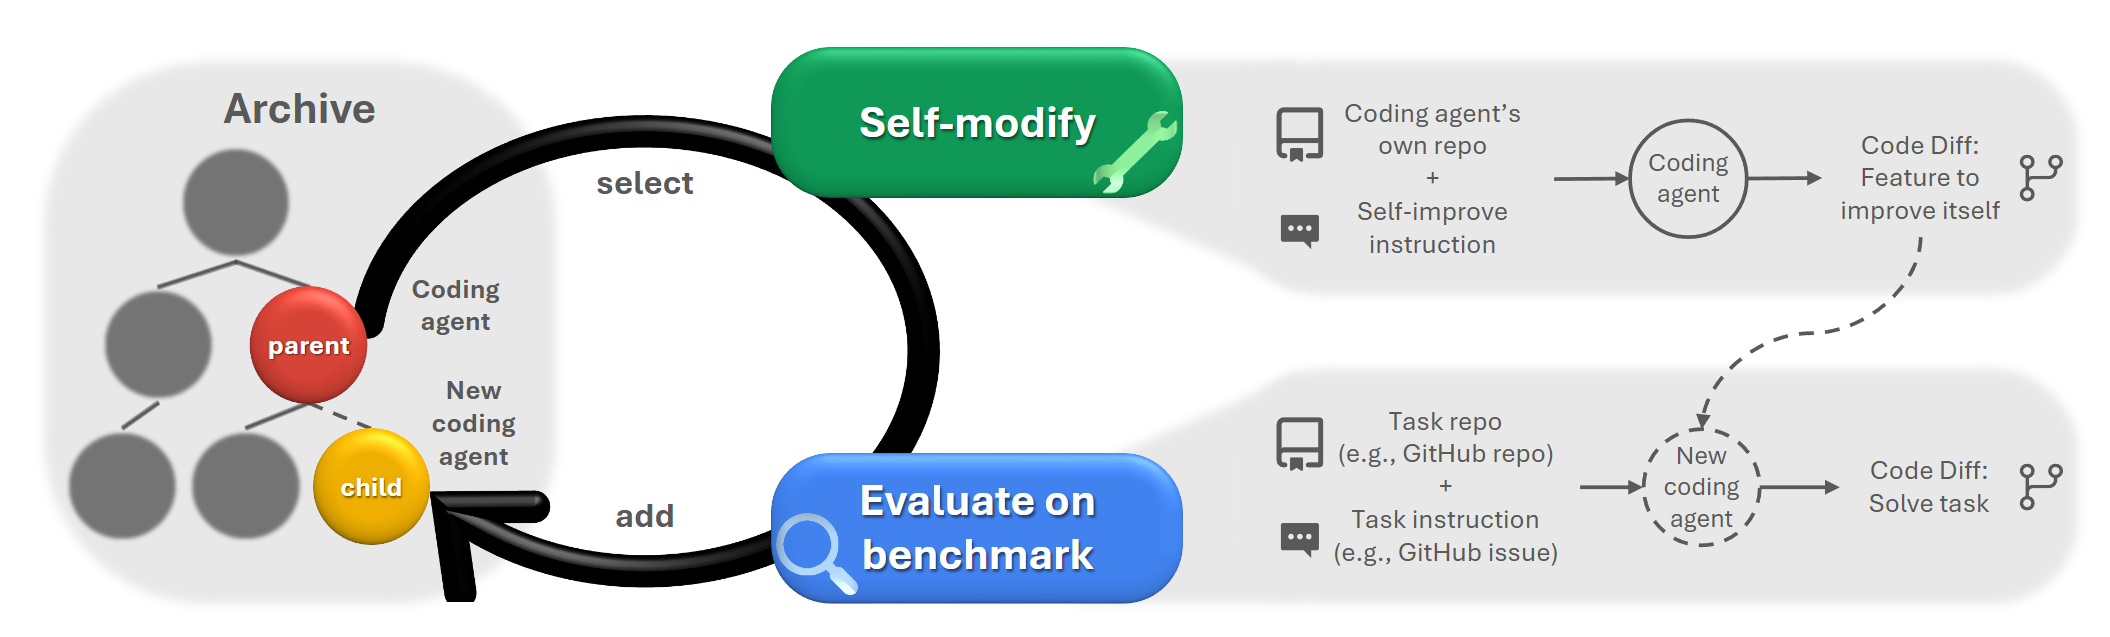
\includegraphics[width=1\textwidth]{images/dgm.png}
    
\end{frame}

\begin{frame}{ShinkaEvolve: Sample-Efficient Program Evolution\\ \liturl{Lange et al. 2025}{https://arxiv.org/abs/2509.19349}}
    \textbf{Algorithmic Idea:}
    ShinkaEvolve addresses the sample inefficiency of previous code evolution methods by introducing new sampling and selection mechanisms to balance exploration and exploitation.

    \pause
    \vspace*{0.5cm}
    \textbf{Key Mechanisms:}
    \begin{itemize}
        \item \textbf{Novelty Rejection-Sampling:} Prevents the LLM from redundantly exploring the same search space by rejecting semantically identical or overly similar code candidates.
        \pause
        \item \textbf{Bandit-Based LLM Ensemble:} Dynamically allocates generation budget among a diverse ensemble of LLMs using Multi-Armed Bandit strategies to maximize the quality of mutated programs.
    \end{itemize}
    
\end{frame}

\begin{frame}{ShinkaEvolve: Sample-Efficient Program Evolution\\ \liturl{Lange et al. 2025}{https://arxiv.org/abs/2509.19349}}

    \centering
    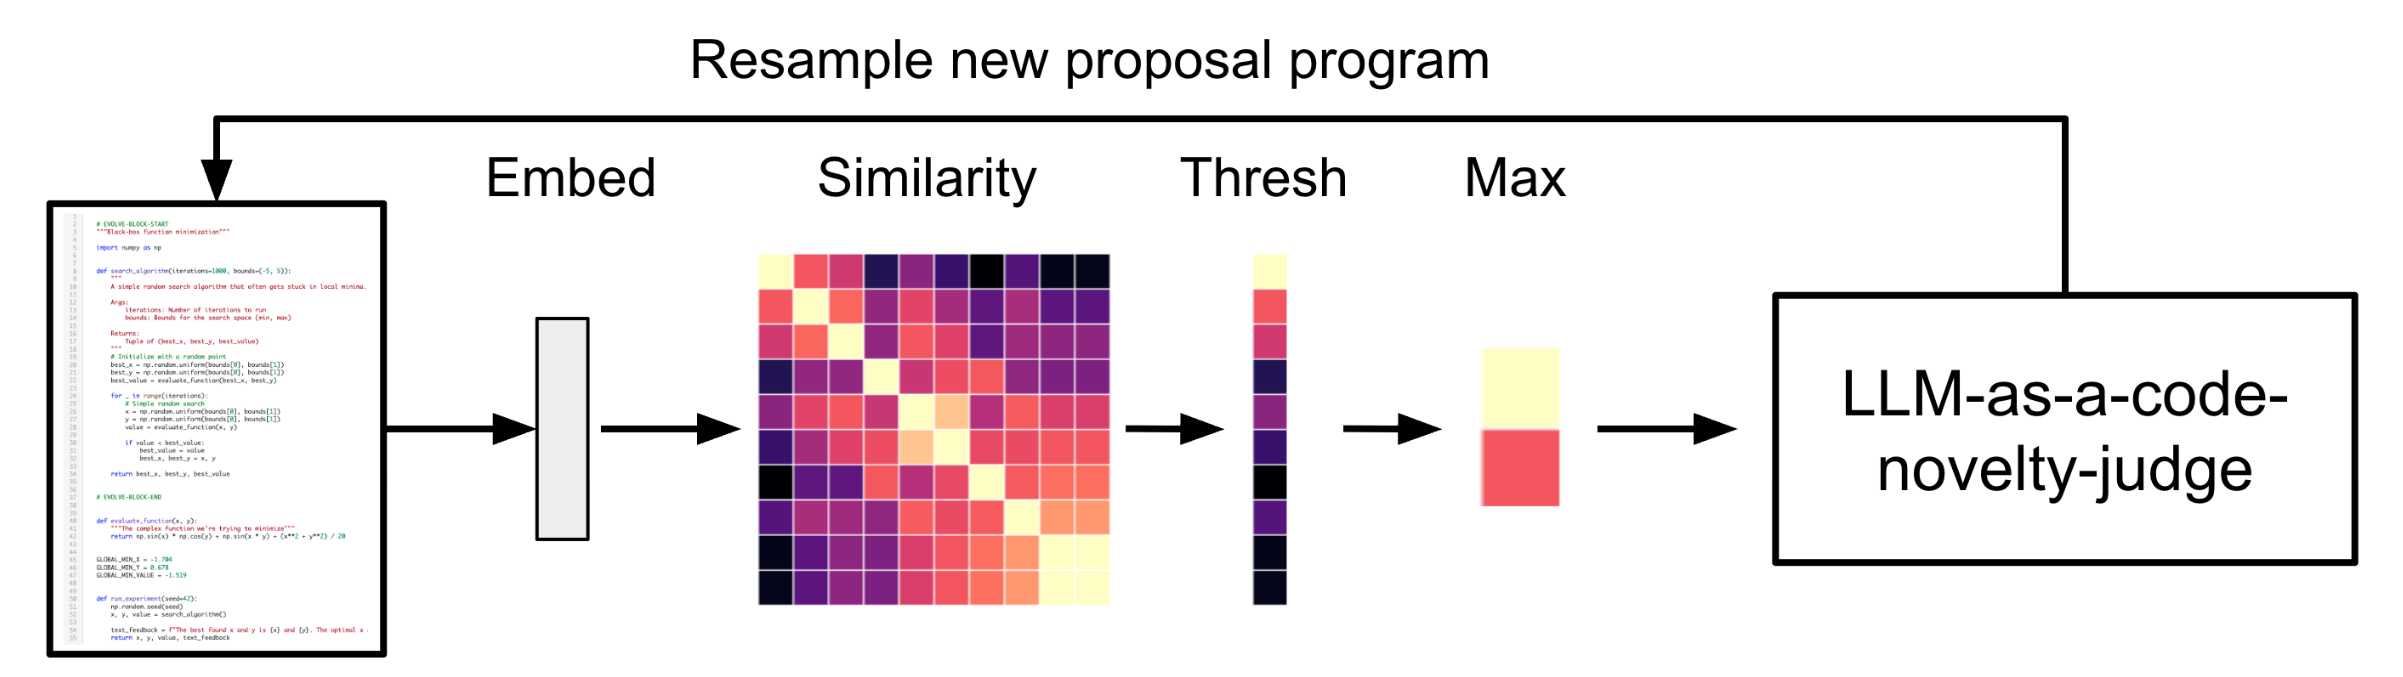
\includegraphics[width=1.0\textwidth]{images/shinka.png}
    ``ShinkaEvolve embeds mutable code snippets, computes similarities across the archive; if the maximal score exceeds a threshold, another LLM is queried to assess whether the program is meaningfully novel.''
    
\end{frame}



\begin{frame}{LLaMEA: LLM Evolutionary Algorithm \liturl{van Stein and Bäck et al. 2024}{https://arxiv.org/pdf/2405.20132}}
    \textbf{Algorithmic Idea:}
    LLaMEA framework specifically targets the automated generation of metaheuristic optimization algorithms (e.g., EAs or BO~\liturl{Li et al. 2025}{https://arxiv.org/abs/2505.21034}). It iteratively designs, evaluates, and refines optimization algorithms tailored for given optimization tasks.

    \pause
    \textbf{Key Mechanisms:}
    \begin{itemize}
        \item \textbf{Task Definition:} The LLM receives a prompt outlining the algorithm structure (e.g., initialization, step generation, selection).
        \pause
        \item \textbf{Iterative Refinement:} Generates new metaheuristics, evaluates them on benchmark suites (like BBOB), and feeds the performance metrics back as a prompt to the LLM.
        \pause
        \item \textbf{HPO:} Hyperparameter optimization (on the meta-level) can be taken care by either the LLM or by an external tool (such as SMAC or Optuna)
    \end{itemize}
    
    
\end{frame}

\begin{frame}{Synthesis: The LLM-Evolutionary Paradigm}
    \textbf{Common Thread:}
    Across all methods, the fundamental paradigm treats code generation as an evolutionary search problem, with the LLM serving as the source of variation.

    \pause
    \textbf{Core Components:}
    \begin{enumerate}
        \item \textbf{Representation:} Solutions are represented as executable code (Python functions, classes).
        \pause
        \item \textbf{Variation (LLM):} LLMs execute semantic mutations, crossovers, and heuristic generation guided by prompts.
        \pause
        \item \textbf{Evaluation:} Sandboxed execution against benchmarks, mathematical evaluators, or simulated environments.
        \pause
        \item \textbf{Selection:} Archiving, island models, or bandit algorithms to maintain high-fitness and diverse code bases.
    \end{enumerate}
    
\end{frame}

\begin{frame}{Summary}
    \begin{itemize}
        \item \textbf{Generative Models as Optimizers:} Pre-trained models can transcend their training data by acting as intelligent search operators in a larger iterative framework.
        \pause
        \item \textbf{Verifiable Output:} While LLMs may hallucinate, coupling them with programmatic evaluators ensures that only verifiable, high-quality discoveries are retained.
        \pause
        \item \textbf{Continuous Self-Improvement:} The trajectory of modern AI systems is shifting from static, human-designed architectures towards open-ended, self-modifying systems.
        \pause
        \item \textbf{Efficiency through Meta-Strategies:} As the search space of algorithms is vast, incorporating diversity-preservation, novelty search, and meta-learning significantly boosts sample efficiency and the rate of discovery.
    \end{itemize}
    
    
\end{frame}

\end{document}

